\chapter{Methodology}
\label{chap:methodology}

\section{Developement of the simulation model}
\subsection{Specifications}
In order to predict with precision the electrical output of a run-of-the-river power plant, the following parameters and values would be needed : 
\begin{itemize}
\itemsep0em
 \item Power plant parameters : 
 \begin{itemize}
  \item nominal water flow through the turbine ($Q_\mathrm{nenn}$)
  \item nominal head of water ($H_\mathrm{nenn}$)
  \item nominal water level ($W_\mathrm{nenn}$)
  \item efficiency curve of the turbine ($\eta_\mathrm{turbine}$) 
  \item efficiency of the generator ($\eta_\mathrm{generator}$)  
  \item unusable water flow ($Q_\mathrm{rest}$)  
 \end{itemize}
 \item Input time series : 
 \begin{itemize}
  \item actual water flow through the turbine ($Q$)
  \item actual water level downstream from the turbine ($W$)
 \end{itemize}
\end{itemize}

However, if such precise data can be found for single power plants, it is not easily accessible at a state or country-wide level. The OEDB database lists the location and nominal power of the plants, without further information on their design. The german Bundesnetzagentur is developing a register of every energy production facility in Germany, called MaStR (Marktstammdatenregister). This register should give a complete overview of the power plants in Germany, sorted by energy carrier and type of plant (reservoir, run-of-the-river, pumped hydro...), and listing the location and nominal power, as well as the presence or not of a restriction of the usable water flow due to a fish ladder or fish protection system for instance \cite{MaStR}. This last information is not yet available in registers such as the OEDB.\newline
Therefore, the model should be able to extrapolate missing data and to make some assumptions when optional input parameters are not provided. The only compulsory input parameter will be the broadly available nominal power of the turbine and section \ref{missing_data} explains how other parameters can be assumed or extrapolated. \newline
In terms of time series, in addition to the water flow over the simulated period, the model will take as input the water flow over several years in order to extrapolate missing parameters. Section \ref{rel_river_data} will go more in details into the reasons why water level data is not relevant. \\
The desired outputs for the model are electricity production time series per power plant or per area. It should also be possible to simulate several plants in one go.

\subsection{Collection and administration of data basis}

It is estimated that among the 6500 to 7500 hydropower plants in Germany, only 406 have a nominal power above 1MW \cite{uba_wasserkraft}. Out of 7500 run-of-the-river hydropower plants in the OpenEnergy Database, 5600 have a capacity under 100kW (see figure \ref{oedb_capa} in section \ref{hpp_register}).  However, the plants under 1MW account for a small part of the total installed power (see figure \ref{uba_hpp}). For that reason, the generator efficiency has been approximated to 95\% for all power plants is this work.

\begin{figure}[H]
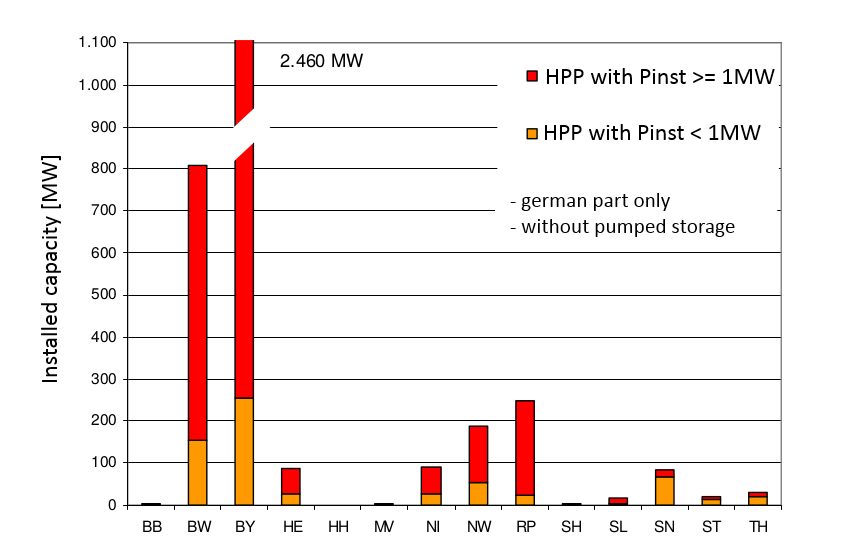
\includegraphics[width=15cm]{uba_hpp_en.png}
\caption[Installed power pro Bundesland for plants over and under 1MW]{Installed power pro Bundesland for plants over and under 1MW \cite{uba_wasserkraft}}
\centering
\label{uba_hpp}
\end{figure}
XXX take some from above and complete : inputs, parameters and validation data
XXX write here the stuff about W not being relevant

For this reason, the state-wide simulation of hydropower production presented in the case study from section XXX UPDATE WHEN READY XXX as been conducted for XXX TH or ST or MV XXX, in order to compare the results of the simulation based on the OEDB register with the yearly production values given by the AEE.

In this work, data from the BfG was used as input to test the model (XXX put references of teil über Mosel und Thuringe XXX), as well as data from the french ``Banque Hydro'' (XXX reference of the teil über Hydroraon XXX). The ``Banque Hydro'' is run by the SCHAPI (Service Central d'Hydrométéorologie et d'Appui à la Prévision des Inondations), a section of the french Ministry of Ecology, Sustainable Development and Energy, and gathers data from around 5000 gauge stations.


\subsection{Simulation results and evaluation}
XXX Over which period of time, stepsize, error...

\section{Data preprocessing}

\subsection{Power plants register - OEDB}
XXX GIS/SQL code from Ludwig. Next neighbour finden, gauge station has to be on the same river...
\subsection{Runoff data}
XXX structure in DB

\section{Simulation}

\section{Evaluation of results}

